% -*- coding: utf-8 -*-

\chapter{Estado del arte y trabajos relacionados}
\label{chap:antecedents}
\drop{E}{n} el siguiente capítulo se realiza una presentación de los conceptos y
tecnologías que han sido utilizadas para la elaboración del proyecto y se hace
un repaso de algunos de los trabajos y aplicaciones reales que han servido de
inspiración para el diseño final del sistema.

\section{Estado del arte}
A continuación, se citan los principales elementos que constituyen la base
teórica sobre la que se sustenta el resto del escrito.

  \subsection{La tecnología \acs{RFID}}
\acs{RFID} son las siglas de \emph{Radio Frequency IDentification} (en
castellano, \emph{\textbf{identificación por radiofrecuencia}}). Se trata de un
sistema de almacenamiento y recuperación de datos remoto que utiliza las ondas
de radio para transmitir la identidad (única) de un objeto.

El modo de funcionamiento de los sistemas \acs{RFID} es simple. Una
\textbf{etiqueta \acs{RFID}} (o transponedor) que contiene datos genera una
señal de radiofrecuencia con dichos datos. Esta señal es captada por un
\textbf{lector \acs{RFID}} y este la transforma a una señal digital entendible
por una aplicación específica que utilice \acs{RFID} (figura
\ref{fig:rfidSystem}).

\begin{figure}[!h]
  \begin{center}
    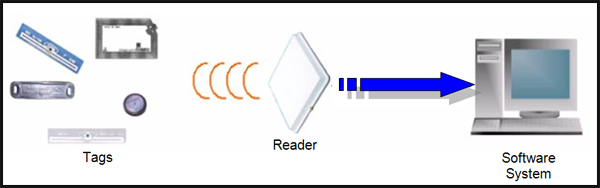
\includegraphics[width=0.8\textwidth]{rfidSystem.png}
    \caption{Esquema básico de un sistema \acs{RFID}.}
    \label{fig:rfidSystem}
  \end{center}
\end{figure}

    \subsubsection{Historia}
  El origen del \acs{RFID} está relacionado con la II Guerra Mundial. Los
  radares de la época eran capaces de detectar y medir la presencia de objetos
  dentro de un rango de actuación, pero no eran capaces de identificar qué
  clase de objetos eran identificados.

  Durante la década de los 50 y los 60, científicos de los países más
  avanzados, trabajaron para explicar cómo podrían identificar objetos
  remotamente. Fruto de estos estudios se inventaron los primeros sistemas
  antirrobo que funcionaban con ondas de radio. El objeto en cuestión tenía 
  una etiqueta con un único bit que decía si el artículo se había pagado o no.
  Cuando el objeto había sido pagado, se modificaba dicho bit, para que los 
  sensores de la salida no accionaran la alarma.

  Las primeras patentes fueron solicitadas en Estados Unidos en 1973. Mario W.
  Cardullo presentó una etiqueta \acs{RFID} activa que portaba una memoria
  rescribible. Y ese mismo año, Charles Walton recibió la patente para un
  sistema \ac{RFID} pasivo, consistente en una tarjeta con un transponedor que
  comunicaba una señal a un lector situado en una puerta. Si la tarjeta era
  validada por el lector, se desbloqueaba la cerradura de la puerta.

  A partir de ese año, la tecnología \acs{RFID} empezó a utilizarse por ejemplo,
  en sistemas de apertura de puertas automáticas en centrales nucleares o en
  sistemas para controlar el ganado que había sido vacunado y el que no.

  En la década de los 90, el desarrollo de nuevos materiales permitió
  reducir drásticamente el precio de las etiquetas. Este hecho favoreció
  que se potenciara el número de aplicaciones que utilizan esta tecnología.
  Es por ello que organismos internacionales empezaran a poner sus esfuerzos en
  desarrollar estándares en el uso de este tipo de etiquetas.

    \subsubsection{Etiquetas \acs{RFID}. Arquitectura y funcionamiento}
  Las etiquetas \acs{RFID} son dispositivos pequeños, similares a una pegatina,
  que pueden incorporarse a un objeto, un animal o una persona. 
  
  Todas las etiquetas \acs{RFID} tienen en común los siguientes elementos
  (figura \ref{fig:rfidComponents}):

  \begin{figure}[!h]
    \begin{center}
      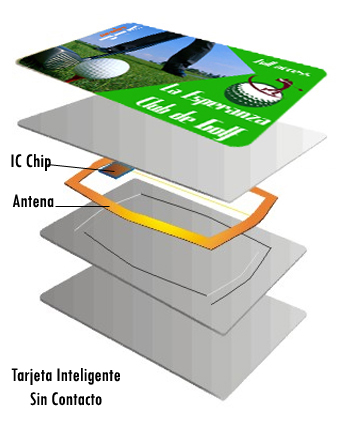
\includegraphics[width=0.4\textwidth]{rfidComponents.png}
      \caption{Componentes de una tarjeta \acs{RFID}.}
      \label{fig:rfidComponents}
    \end{center}
  \end{figure}

  \begin{itemize}
    \item \textbf{Antena}. Se encarga de recibir las señales emitidas por el
  lector y de enviar la respuesta ante dichas señales.
    \item \textbf{Chip}. Contiene la lógica de operación de la etiqueta y un
  número de identificación único.
    \item \textbf{Memoria}. Está compuesta por una parte de sólo lectura,
  que contiene las instrucciones básicas para el funcionamiento de la etiqueta;
  y por una parte de lectura y escritura, que almacena los datos escritos
  durante una comunicación con el lector.
  \end{itemize}
  
  Por otro lado, las etiquetas \ac{RFID} pueden ser de tres tipos:
  \begin{itemize}
    \item \textbf{Pasivas}. No poseen ninguna fuente autónoma de energía. La
  señal del lector es la que le induce una pequeña cantidad energía suficiente 
  como para generar y transmitir la respuesta. Tienen una fiabilidad y una
  capacidad de almacenamiento muy limitadas (unos pocos KBytes) y su campo de
  cobertura es también muy reducido (hasta 3 metros). Aún así, son las más
  utilizadas debido a su bajo coste.
   \item \textbf{Activas}. Poseen su propia fuente autónoma de energía y la
  utilizan para dar corriente a sus circuitos integrados y para propagar su
  señal al lector. Esto implica que las comunicaciones son más fiables (tienen
  menos errores), pueden transmitir señales más potentes y a mayor distancia
  (hasta 500m) y tienen más capacidad de almacenamiento. Por otro lado, tienen
  un mayor coste por chip y son de mayor tamaño que las etiquetas pasivas. La
  vida útil de sus baterías puede llegar hasta los 10 años.
    \item \textbf{Semipasivas}. Al igual que las etiquetas activas, las
  semipasivas también disponen de una fuente autónoma de energía. Sin embargo,
  estas utilizan la energía principalmente para alimentar el chip, no para
  transmitir la señal. Tienen una fiabilidad comparable a la de las etiquetas
  activas aunque superan su vida útil. Por otro lado, tienen un rango
  operativo comparable a las etiquetas pasivas aunque su respuesta es más
  rápida.
  \end{itemize}

    \subsubsection{Lectores RFID. Funcionamiento}
  Los lectores \acs{RFID} son los encargados de leer o re-escribir la
  información almacenada en las etiquetas.
  El funcionamiento es sencillo. La antena del lector crea un campo magnético
  y cuando este campo entra en contacto con una etiqueta, se produce la
  reacción de esta última, enviando al lector la información contenida.
  El lector decocifica los datos obtenidos y los manda a una tercera entidad 
  para que los interprete (figura \ref{fig:rfidSchema}).

  \begin{figure}[!h]
    \begin{center}
      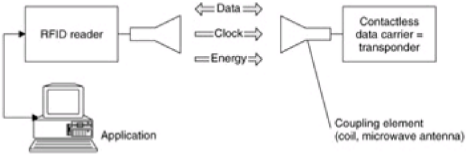
\includegraphics[width=0.8\textwidth]{rfidSchema.png}
      \caption{El lector y la etiqueta son los principales componentes de todo
sistema \acs{RFID}.}
      \label{fig:rfidSchema}
    \end{center}
  \end{figure}

  Según el número de bobinas que poseen, existen dos tipos de lectores:
  \begin{itemize}
  \item \textbf{Bobina simple}. La misma bobina crea el campo magnético y
  transmite los datos. Son más simples y baratas que las dobles y tienen
  un alcance muy limitado.
  \item \textbf{Bobina doble}. Una de las bobinas se encarga de crear el
  campo magnético y la otra de transmitir los datos. Son caras pero tienen
  mayores prestaciones que las bobinas simples.
  \end{itemize}
  
  En cuanto a la portabilidad, también existen dos tipos de lectores:
  \begin{itemize}
  \item \textbf{Lectores móviles}. Son lectores autónomos que pueden 
  transportarse a cualquier lugar y que pueden utilizarse con varios fines. Se
  comunican con otros dispositivos a través de conexiones inalámbricas.
  \item \textbf{Lectores fijos}. Son lectores ubicados en un punto fijo y 
  dedicados a un único fin. Tienen mayor rango de actuación que los lectores
  móviles y suelen utilizarse en sistemas de detección y seguimiento de
  personas y animales.
  \end{itemize}

    \subsubsection{La tecnología \emph{MIFARE}}
  \emph{MIFARE} es el estándar de la industria para interfaces de
  tarjetas inteligentes sin contacto y lectores que operan a 13.56MHz.
  Funcionan de acuerdo con el estándar \acs{ISO} 14443\cite{bib:mifare}.
  
  El alcance típico de lectura/escritura de etiquetas \emph{MIFARE} sin
  contacto oscila entre los 2 y los 10 cm; y la capacidad más habitual está
  entre los 1 y los 4KB de memoria \acs{EEPROM}.

  Para que los datos sean leídos o escritos es necesaria una autentificación 
  mútua entre el lector y la etiqueta, ya que el acceso a los mismos está 
  protegidos por una clave de 48 bits. La transmisión de datos por
  radiofrecuencia viaja encriptada.

  En la actualidad \emph{MIFARE} es una marca registrada de \emph{NXP
  Semiconductors} (empresa fundada por \emph{Philips}). Ha vendido más de 5 mil
  millones de tarjetas y etiquetas inteligentes y más de 50 millones de
  componentes de lectores. Ha sido seleccionada para la mayoría
  de proyectos importantes con tarjetas inteligentes sin contacto en todo el
  mundo y su cartera de productos incluye soluciones perfectas para la
  recaudación automática de tarifas, tarjetas de fidelización, cobro en 
  carreteras de peaje o gestión de acceso a edificios\cite{bib:urlMifare} 
  (figura \ref{fig:mifareFamily}).

  \begin{figure}[!h]
    \begin{center}
      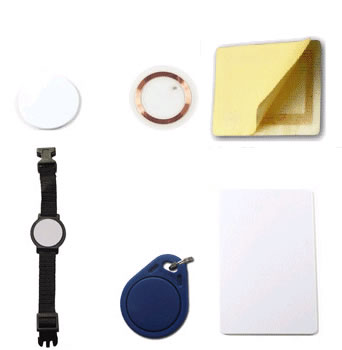
\includegraphics[width=0.5\textwidth]{mifareFamily.png}
      \caption{Ejemplos de etiquetas MIFARE.}
      \label{fig:mifareFamily}
    \end{center}
  \end{figure}

% El chorizo de las siguientes partes lo meteré más adelante...
  \subsection{La tecnología NFC}
%%%%%%%%%%%%%%%%%%%%%%%%%%%%%%
% Pondré más o menos que en el apartado del RFID

  \subsection{La tecnología Bluetooth}
%%%%%%%%%%%%%%%%%%%%%%%%%%%%%%
% Pondré más o menos que en el apartado del RFID

  \subsection{Los servicios web}
%%%%%%%%%%%%%%%%%%%%%%%%%%%%%%
% Ya veré que se me ocurre meter aquí, porque no hay mucho que explicar

  \subsection{El framework .NET}
%%%%%%%%%%%%%%%%%%%%%%%%%%%%%%
% No sé si meterlo

  \subsection{La tecnología Java}
%%%%%%%%%%%%%%%%%%%%%%%%%%%%%%
% Explicación muy general supongo

  \subsection{Los displays táctiles}
%%%%%%%%%%%%%%%%%%%%%%%%%%%%%%
% Explicación superficiar supongo, nada de cómo funcionan pero sí de donde
% y porqué se usan

  \subsection{La computación móvil}
%%%%%%%%%%%%%%%%%%%%%%%%%%%%%%
% Tema super-amplio, tendré que decir la evolución y para qué se usan 
% últimamente

\section{Trabajos relacionados}
  \subsection{Estudios relacionados}
  \label{subsec:related}
    \subsubsection{Modelos de comercio utilizando NFC}
  Los servicios que ofrece \acs{NFC} están muy diversificados y extendidos
  por todo el mundo. Algunos de los servicios están orientados a utilizar
  las tarjetas inteligentes como un monedero electrónico sustitutivo del
  pago en efectivo en los medios de transporte público, otros sustituyen
  a los clásicos cupones para premiar la fidelidad de los clientes de un
  establecimiento, otros sirven para solicitar un servicio de entre una
  lista de servicios disponibles (como elegir un producto dentro de una
  lista de productos), etc.

  Con el fin de integrar todos estos servicios como un proceso común de
  comercio electrónico basado en NFC, se ha propuesto un modelo genérico
  para el comercio móvil basado en \acs{NFC} (o \acs{NMC}, por sus siglas
  en inglés) \cite{bib:nfcCommerce}. Este modelo caracteriza los problemas y
  las tecnologías que intervienen en cada una de las siguientes fases
  (figura \ref{fig:nmcModel}):

  \begin{figure}[!h]
    \begin{center}
      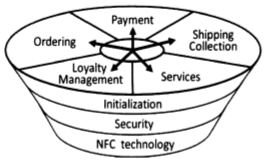
\includegraphics[width=0.5\textwidth]{nmcModel.png}
      \caption{El modelo \acs{NMC}.}
      \label{fig:nmcModel}
    \end{center}
  \end{figure}

  \begin{itemize}
  \item \textbf{Fase de inicialización}. Para la construcción de un servicio
  de comercio basado en \acs{NFC} se necesitan definir cuatro componentes
  fundamentales:
    \begin{itemize}
    \item \textbf{Servicio de \emph{back-end}}\footnote{En diseño de software
    el \emph{front-end} es la parte del software que interactúa con el o los
    usuarios y el \emph{back-end} es la parte que procesa la entrada desde el
    \emph{front-end}} \textbf{basado en \acs{NFC}}. Este
    servicio es el responsable de todo el intercambio de información durante
    el proceso de comercio. Está gestionado por el proveedor de servicios
    basados en \acs{NFC}.
    \item \textbf{Aplicación de terminal genérico (\acs{GTA})}. Como el tamaño
    de la memoria del dispositivo móvil es limitada, combiene definir una
    aplicación genérica que permita realizar todas las gestiones comerciales.
    \item \textbf{Funcionalidad de las etiquetas}. Definir los tipos de
    etiquetas que se utilizarán para construir un entorno de servicios con
    \acs{NFC} que siga el estándar \acs{NDEF}. Por ejemplo, un tipo de etiqueta
    para iniciar la aplicación, otro para cada uno de los productos, otro
    para seleccionar descuentos y otro para seleccionar el servicio.
    \item \textbf{Habilitar el servicio \acs{NFC}}. La etiqueta de inicio de
    aplicación se encargará de cargar el \acs{GTA} y de arrancar el servicio de
    \emph{back-end}, para que el usuario pueda usarlos nada más iniciar la
    aplicación.
    \end{itemize}
  \item \textbf{Fase de pedido}. Después de la inicialización el cliente ya
  está preparado para realizar un pedido a través de un catálogo de productos:
    \begin{itemize}
    \item Cada \textbf{catálogo} tiene una o varias etiquetas que representan
    los productos ofrecidos por el servicio. Cuando el dispositivo toca una
    de estas etiquetas, la aplicación puede llamar al servicio \emph{back-end}
    para descargar el contenido (imágenes, videos, etc.) relacionado con el
    contenido del producto al que representa la etiqueta.
    \item Además, cada producto puede tener opciones del tipo \emph{sabor},
    \emph{volumen}, \emph{tamaño}; que pueden ser seleccionables a través
    de otras etiquetas o a través de la pantalla del dispositivo.
    \end{itemize}
  \item \textbf{Fase de pago}. Hay dos métodos de pago disponibles en el
  modelo \acs{NMC}:
    \begin{itemize}
    \item \textbf{Modo monedero electrónico} (figura \ref{fig:e-wallet}). 
    Después de que el cliente haya realizado un pedido, el \acs{GTA} 
    solicitará la información del producto al servicio \emph{back-end}. Si el 
    servicio \emph{back-end} confirma la autenticidad del usuario y de la 
    operación, le devolverá al \acs{GTA} el importe del producto. Esta 
    cantidad será decrementada del monedero electrónico. El monedero 
    electrónico es un elemento seguro al que sólo se puede acceder con el 
    permiso del servicio \emph{back-end}. Los clientes deben disponer de saldo 
    para poder realizar un pedido (método prepago).

    \begin{figure}[!h]
      \begin{center}
        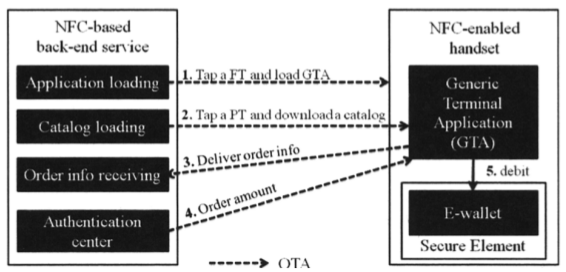
\includegraphics[width=0.5\textwidth]{e-wallet.png}
        \caption{Fase de pago con \emph{modo monedero electrónico}.}
        \label{fig:e-wallet}
      \end{center}
    \end{figure}

    \item \textbf{Modo tarjeta de crédito} (figura \ref{fig:creditCard}). 
    Antes de utilizar este modo para llevar a cabo la transacción, el banco 
    debe facilitar al cliente un \emph{applet\footnote{Componente de una 
    aplicación que se ejecuta en el contexto de otro programa. No puede 
    ejecutarse de manera independiente.}} que tiene que ser cargado en el 
    dispositivo móvil. Una vez realizado el pedido, el \acs{GTA} almacena el 
    número de orden como elemento seguro. Para realizar el pago, el cliente 
    aproxima el dispositivo móvil al lector del comerciante y este lee el 
    número de orden almacenado. El servicio de \emph{back-end} comprueba el 
    importe a pagar y se inicia un intercambio de información entre el lector 
    del banco y el \emph{applet} de la tarjeta de crédito. Por último, el 
    lector del banco obtiene el código de autorización para finalizar la 
    transacción.
  
    \begin{figure}[!h]
      \begin{center}
        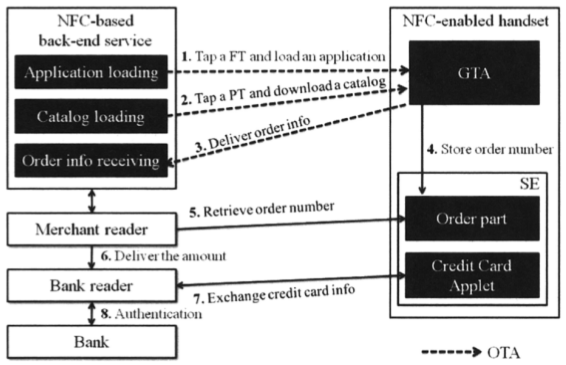
\includegraphics[width=0.5\textwidth]{creditCard.png}
        \caption{Fase de pago con \emph{modo tarjeta de crédito}.}
        \label{fig:creditCard}
      \end{center}
    \end{figure}

    \end{itemize}
  \item \textbf{Fase de envío y recogida}. En esta fase, el cliente elige
  la forma y el lugar en que recibe el producto o servicio. Para productos
  físicos elegirá el lugar al que deben llevárselo o el lugar en el que quiere
  recogerlo. Y para productos virtuales el dispositivo donde quiere
  almacenarlo.
  \item \textbf{Fase de gestión de fidelización}. El programa de fidelización
  está diseñado para incentivar al cliente a consumir de nuevo. Los cupones son
  herramientas de fidelización comunes y la tecnología \acs{NFC} hace factible
  el concepto de \emph{cupones virtuales}.
    \begin{itemize}
    \item Los clientes pueden recibir cupones tocando una etiqueta que 
    simbolice la descarga de un cupón.
    \item A través de \acs{NFC}, utilizando el modo de comunicación
    \emph{peer-to-peer}, los clientes pueden compartir sus cupones con los
    demás. Esto puede aprovecharse para desarrollar un programa de
    \emph{márketing} atractivo y eficaz.
    \end{itemize}
  \item \textbf{Fase de servicio}. Para solicitar un servicio bastará con
  tocar con el dispositivo móvil una etiqueta de tipo servicio. Las diferentes
  opciones de servicio que estén disponibles serán accesibles a través de
  otras etiquetas de servicio o mediante la selección de ese servicio en la
  pantalla del dispositivo.
  \end{itemize}
  
  Dada su generalidad, el modelo basado en el comercio móvil \acs{NMC} está 
  pensado para establecer las líneas maestras a la hora de desarrollar 
  cualquier clase de servicios móviles; entre ellos por supuesto, un sistema
  de gestión de restaurantes basado en \acs{NFC}.

    \subsubsection{Métodos de pago móvil a distancia}
  Hoy en día se pueden distinguir dos tipos de pagos a distancia: los que se
  producen de forma remota, como cuando se realizan compras por internet;
  y los que se realizan dentro del mismo sitio donde se está
  comprando. El primero de ellos goza de una gran popularidad, ya que se
  considera un método fácil, cómodo y bastante seguro; y no requiere de una
  infraestructura especial para ser implementado. El segundo en cambio,
  aún no goza de la misma aceptación, debido en parte a que los 
  establecimientos no están dispuestos a invertir su dinero en adquirir una 
  infraestructura adicional para permitir este tipo de pagos, sin ver antes 
  que hacerlo les reporte algún tipo de beneficio.

  En la actualidad el pago a distancia por móvil utilizando la tecnología
  \acs{RFID} y \acs{NFC} se puede conseguir mediante uno de estos tres métodos:
  \begin{description}
  \item[SIMpass]. Es una tecnología de interfaz dual que combina la
  tradicional tarjeta \acs{SIM} y la tarjeta \acs{RFID}, en una sola tarjeta
  estándar. La interfaz de contacto cumple con la norma \acs{ISO} 7816 y la
  interfaz a distancia cumple con el estándar de la norma \acs{ISO} 14443.
  \emph{SIMpass} trabaja con una frecuencia de 13,56MHz. Como no es una
  frecuencia muy alta, es difícil minimizar el tamaño de antena. Existen dos
  maneras de implementar dicha antena. Una, de bajo coste, se lleva a cabo 
  utilizando una antena plana que consta de una bobina y que se une a la 
  del teléfono móvil. Para la otra, hay que reformar parte del hardware del 
  teléfono móvil, aunque mejora notablemente la estabilidad y fiabilidad de la
  funcionalidad \acs{RFID}.

  \item[NFC]. Como se ha visto en secciones anteriores, \acs{NFC} es una
  tecnología que combina la tecnología \acs{RFID} con las comunicaciones de
  corto alcance. En el sistema \acs{NFC} propuesto se distinguen tres partes 
  principales: el controlador, la antena y una unidad de seguridad. La unidad
  de seguridad puede correr a cargo de la tarjeta \acs{SIM} o de la tarjeta
  \acs{SD}. El problema está en que, tanto en un caso como en otro, habría que 
  integrar un módulo o chip de seguridad que no viene por defecto en estas 
  tarjetas. Esto se soluciona utilizando la tecnología \acs{NFC} mejorada 
  (\emph{eNFC}). Aunque \emph{eNFC} hace uso de la tarjeta \acs{SIM}, sólo 
  tiene que utilizar el pin C6 para poder modificar la memoria \emph{EEPROM}, 
  en vez de tener que utilizar dos pines (C4 y C8) que además interferirían a 
  la hora de realizar otras operaciones.

    \item[Programa RF-SIM]. Combinando el módulo de comunicaciones móviles y
  los micro-módulos de radio frecuencia (\emph{RF}) de la tarjeta \acs{SIM}
  normal, la tarjeta \emph{RF-SIM} consigue operar a 2,4GHz (una alta 
  frecuencia que tiene una longitud de onda corta). Esto permite que, a través
  de una antena, el módulo \emph{RF-SIM} pueda comunicarse con otros 
  dispositivos externos a distancias entre los 10 y los 500cm, a pesar de que
  dicho módulo tenga un tamaño muy reducido. \emph{RF-SIM} es un tipo de
  etiqueta activa, por lo que necesita una batería para trabajar.
  \end{description}

%%%%%%%%%%%%%%%%%%% He leído hasta aquí %%%%%%%%%%%%%%%%%%%%%%%%%%%%%%%%
%%%%%%%%%%%%%%%%%%%%%%%%%%%%%%%%%%%%%%%%%%%%%%%%%%%%%%%%%%%%%%%%%%%%%%%%

  Cada uno de estos métodos tiene sus ventajas e inconvenientes. Por ejemplo:
  \begin{itemize}
  \item Para implementar el método \emph{SIMpass} es necesario utilizar los
  pines \emph{C4} y \emph{C8}, que están reservados para la interfaz de alta
  velocidad de la tarjeta \acs{SIM}. Por lo tanto tiene un conflicto en la
  evolución futura de la tarjeta \acs{SIM}. Además, aunque la antena que
  necesita tiene un costo más asequible; la fiabilidad, el alcance y la
  velocidad de las transacciones dejan mucho que desear. Por lo que se 
  considera un método poco recomendable.
  \item La distancia de reacción es el factor más significativo de un sistema
  \acs{RFID}. Para un sistema de pago, cuanto más corta sea esta distancia
  más segura será la transacción. El programa \emph{RF-SIM} trabaja a 2.4GHz,
  lo que implica que la distancia de reacción sea demasiado larga como para ser
  segura. Los sistemas inalámbricos \emph{Bluetooth}, \emph{Zigbee}
  \footnote{Especificación de un conjunto de protocolos de alto nivel de 
  comunicación inalámbrica para su utilización con radiodifusión digital de 
  bajo consumo, basada en el estándar IEEE 802.15.4 de redes inalámbricas de 
  área personal. Su objetivo son las aplicaciones que requieren comunicaciones 
  seguras con baja tasa de envío de datos y maximización de la vida útil de 
  sus baterías, como las aplicaciones domóticas.},
  \acs{WiFi} o \acs{UWB}\footnote{Cualquier tecnología de radio que usa un
  ancho de banda mayor de 500 MHz o del 25\% de la frecuencia central, de 
  acuerdo con la FCC (Federal Communications Commission).} usan la misma 
  frecuencia, lo que puede generar interferencias.
  \item El sistema \emph{NFC-SIM} tiene el mismo problema con los pines que
  \emph{RF-SIM} y \emph{NFC-SD} es una solución demasiado costosa.
  \item \emph{eNFC} se plantea como la solución óptima para resolver todos los
  problemas.
  \end{itemize}

  Como se decía, aunque muchos analistas e ingenieros hablan de que los 
  pagos mediante \acs{NFC} sustituirán a los pagos realizados por medios
  tradicionales, esta tecnología aún no es muy común en los teléfonos. En
  Estados Unidos, sólo dos modelos han incluido el hardware \acs{NFC}
  que soporta el pago mediante \emph{Google Wallet}\footnote{Sistema de pago 
  móvil desarrollado por \emph{Google} que permite a los usuarios guardar las 
  tarjetas de crédito, tarjetas de fidelización y tarjetas de regalo, entre 
  otras cosas. Soporta el uso de \acs{NFC}.}. En 2012 se ha anunciado
  la salida de más de 100 modelos con funcionalidad \acs{NFC} (doblando las 
  cifras del 2011). Pero sólo con la producción de más teléfonos con \acs{NFC} 
  no es suficiente. Las tiendas tienen que añadir lectores \acs{NFC} a todas
  sus cajas registradoras y los minoristas no quieren gastar dinero en esto
  hasta que la demanda no sea significativa. Por ello, mientras que esto 
  ocurre, han aparecido nuevas formas de pago que aprovechan las 
  características de otras tecnologías con las que cuentan los móviles, como 
  la lectura de códigos \acs{QR}, el acelerómetro o mediante
  \acs{SMS}\cite{bib:noWaiting}.

    \subsubsection{Métodos de fidelización de clientes}
  Uno de los atractivos que puede tener el uso de la tecnología móvil \acs{NFC}
  es el de poder fidelizar a los clientes en el uso de un servicio. Esto es,
  dependiendo de las operaciones realizadas por un cliente con el móvil en un
  establecimiento, este puede ofrecerle productos que tal vez le interesen,
  puede proponerle descuentos por su fidelidad como cliente o puede utilizar
  el historial de todos los clientes para conocer cuáles son las tendencias
  de consumo.
  
  Uno de los últimos sistemas de fidelización que se ha propuesto para sacar 
  partido a la utilización del \acs{NFC} es \emph{\textbf{WingBonus}}.

  \emph{\href{http://wingbonus.com/}{WingBonus}} es un sistema de
  gestión de promociones formado por una aplicación web y una aplicación móvil
  (disponible para sistemas \emph{Android}). Ha sido creada por el grupo de 
  investigación ISCBD (Ingeniería del Software, Conocimiento y Base de datos) 
  de la Universidad de Córdoba. Y, aunque por el momento sólo muestra 
  promociones ficticias, tiene por objetivo servir algún día de punto de 
  encuentro entre los clientes y sus marcas favoritas, a través de las 
  promociones ofertadas por estos últimos.
  
  A través de la web, los clientes pueden descargar en su móvil cupones, 
  descuentos o tarjetas de fidelización, que pueden ser utilizados a la hora 
  de realizar un pago con \acs{NFC} en los establecimientos donde tengan 
  vigencia. Es decir, si un cliente tiene un cupón de descuento para cortarse 
  el pelo en una peluquería concreta y al pagar en dicha peluquería utiliza el 
  sistema \acs{NFC}, el precio total a abonar por el corte de pelo se verá 
  decrementado por el cupón de descuento.

  El sistema permite dos tipos de usuarios: el usuario registrado y el usuario
  anónimo. Los cupones disponibles para cata tipo de usuario presentan
  características diferentes. Por ejemplo, habrá cupones en los que las
  empresas se interesen por conocer qué tipo de personas (edad, trabajo,
  estatus, etc) descargan y utilizan este tipo de cupones. Si la empresa no
  se preocupa por esta información, todo el mundo podrá descargar cupones
  como anónimo.

  Todas las ofertas que se ofrecen en la web tienen un periodo concreto de
  disponibilidad dentro del cual el cliente puede hacerse con dicha oferta
  (figura \ref{fig:wingBonusP}). Además, las ofertas tienen un tiempo acotado
  de validez que delimita el periodo en el que puede aplicarse dicha oferta.

  \begin{figure}[!h]
    \begin{center}
      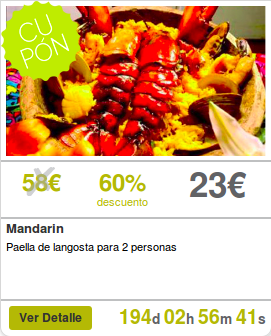
\includegraphics[width=0.5\textwidth]{wingBonusP.png}
      \caption{Ejemplo de cupón ofrecido en la web de \emph{WingBonus}.}
      \label{fig:wingBonusP}
    \end{center}
  \end{figure}

  Los cupones de descuentos tienen la particularidad de que pueden compartirse
  con otros usuarios \acs{NFC} mediante una comunicación \emph{peer-to-peer}.

  Para las empresas asociadas, \emph{WingBonus} ofrece grandes ventajas: 
  reducción de costos, eliminación del papel, poder llegar a más clientes,
  eliminación de las falsificaciones, análisis de mercado, estudio de
  tendencias, fidelización de clientes, etc.\cite{bib:wingBonus}.

  \subsection{Aplicaciones comerciales}
  A continuación, se muestran varios ejemplos de cómo distintos programas
  comerciales implementan las funcionalidades típicas de los gestores de
  restaurantes. Además, también se exponen otras aplicaciones que permiten
  realizar pedidos desde el sitio y sin necesidad de un camarero de ``carne y
  hueso''.

    \subsubsection{Gestión de operaciones típicas de un restaurante}
    En la actualidad existe una innumerable oferta de aplicaciones que ayudan
    a gestionar las labores típicas de un restaurante, como pueden ser:
    gestionar pedidos, generar facturas o realizar la función de caja 
    registradora.

    \begin{itemize}
    \item Para gestionar pedidos las aplicaciones suelen contar con un panel
    de productos en el que se van seleccionando: cantidad, producto y mesa
    a la que va destinado (figuras \ref{fig:productsPanel} y
    \ref{fig:productsPanel2}). Normalmente la iteración consiste en seleccionar
    primero una mesa, seleccionar después la cantidad de productos de un
    mismo tipo y seleccionar por último el producto.

    \begin{figure}[!h]
      \begin{center}
        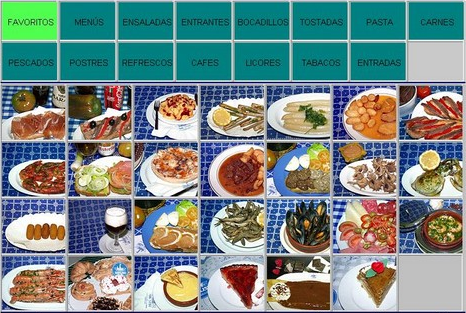
\includegraphics[width=0.8\textwidth]{productsPanel.png}
        \caption{Panel de productos del programa \emph{FrontRest}
        \cite{bib:frontRest}.}
        \label{fig:productsPanel}
      \end{center}
    \end{figure}

    \begin{figure}[!h]
      \begin{center}
        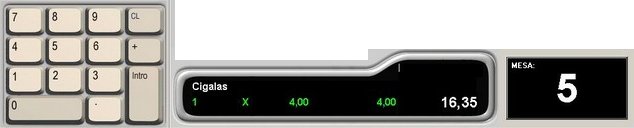
\includegraphics[width=0.8\textwidth]{productsPanel2.png}
        \caption{Panel de selección de cantidad del programa \emph{FrontRest}
        \cite{bib:frontRest}.}
        \label{fig:productsPanel2}
      \end{center}
    \end{figure}

    Una vez terminada la iteración anterior, el pedido queda reflejado en la
    lista de productos asignados a esa mesa (figura \ref{fig:productsList}).

    \begin{figure}[!h]
      \begin{center}
        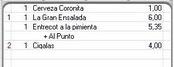
\includegraphics[width=0.5\textwidth]{productsList.png}
        \caption{Lista de pedidos para la mesa 5. \emph{FrontRest}
        \cite{bib:frontRest}.}
        \label{fig:productsList}
      \end{center}
    \end{figure}

    \item A la hora de facturar una mesa, este tipo de aplicaciones suelen
    presentar un resumen con los datos de la mesa a facturar, la lista de
    pedidos realizados, el importe parcial de cada uno de ellos, el importe
    subtotal y el importe total con impuestos incluidos (figura
    \ref{fig:bill}).

    \begin{figure}[!h]
      \begin{center}
        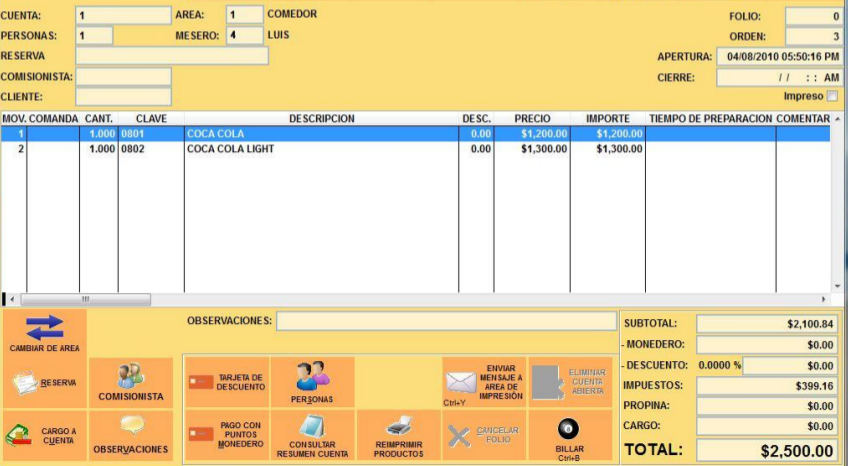
\includegraphics[width=1\textwidth]{bill.png}
        \caption{Resumen de facturación de una mesa en el programa
        \emph{Soft Restaurant}\cite{bib:softRestaurant}.}
        \label{fig:bill}
      \end{center}
    \end{figure}

    Con estos datos, el camarero conoce en tiempo real cuál es la lista de
    productos de una mesa y cuál es el importe total que los comensales deben
    abonar en concepto de los productos consumidos.

    \item Los productos con los que estos programas trabajan, deben ser
    editados por los responsables del restaurante. Entre los atributos que
    estos poseen están: código, nombre, categoría o precio (figura
    \ref{fig:editProduct}).

    \begin{figure}[!h]
      \begin{center}
        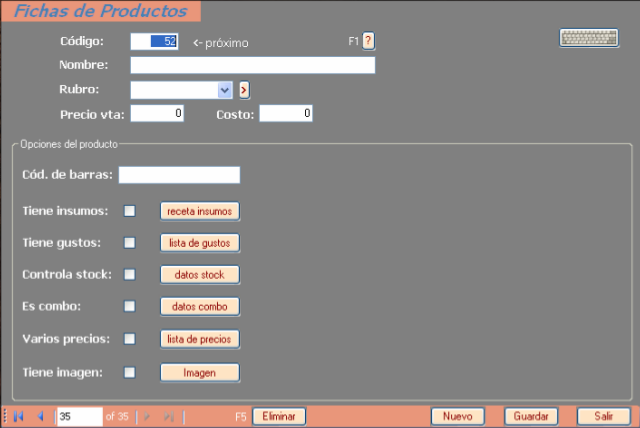
\includegraphics[width=0.8\textwidth]{editProduct.png}
        \caption{Editor de productos del programa \emph{SaleYa}
        \cite{bib:saleYa}.}
        \label{fig:editProduct}
      \end{center}
    \end{figure}
    \end{itemize}

    Estas son las funcionalidades básicas que todo software de 
    gestión de restaurante debe tener. Pero, aparte de estas, son muchas otras 
    las funcionalidades que pueden ayudar a mejorar la gestión de un 
    restaurante.

    \begin{itemize}
    \item Es muy común en casi todos los programas de gestión de restaurantes
    buscar una representación aproximada de las partes que conforman el
    restaurante. En un principio, lo que más interesa representar son las mesas
    que el restaurante contiene, aunque hay aplicaciones que distinguen entre
    la barra, las mesas del salón, las mesas de la terraza y otros objetos
    (figura \ref{fig:tables}).

    \begin{figure}[!h]
      \begin{center}
        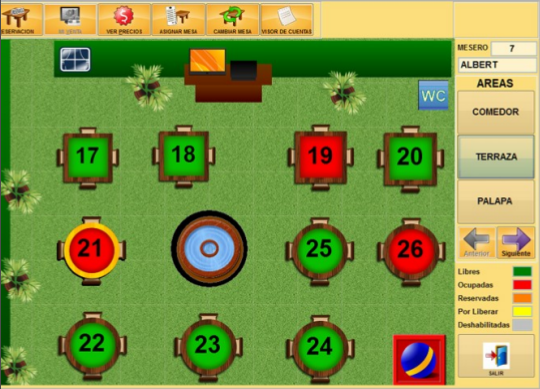
\includegraphics[width=0.8\textwidth]{tables.png}
        \caption{Mapa de un restaurante de la aplicación
        \emph{Soft Restaurant}\cite{bib:softRestaurant}.}
        \label{fig:tables}
      \end{center}
    \end{figure}

    Estos mapas ayudan a los camareros a reconocer el estado en el que se
    encuentran las mesas (ocupadas, libres, reservadas, deshabilitadas, etc.).
    Los símbolos del mapa ayudan a ubicar dónde se encuentran los objetos
    reales a los que representan y su color representa el estado en el que
    se encuentran.

    \item Aplicaciones como \emph{Soft Restaurant}\cite{bib:softRestaurant} o 
    \emph{SaleYa}\cite{bib:saleYa} tienen una funcionalidad que permite 
    describir las recetas de los productos contemplados en la carta. Es decir, 
    permite listar los ingredientes (con sus cantidades) utilizados en la 
    elaboración de cada plato (figura \ref{fig:ingredients}). Esto facilita la
    gestión del \emph{stock} de esos ingredientes.

    \begin{figure}[!h]
      \begin{center}
        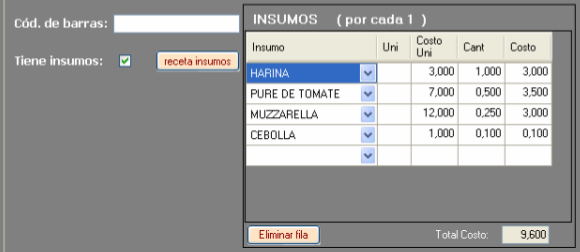
\includegraphics[width=0.8\textwidth]{ingredients.png}
        \caption{Ingredientes para la elaboración de una \emph{pizza de 
        mozzarella}. \emph{SaleYa}\cite{bib:saleYa}.}
        \label{fig:ingredients}
      \end{center}
    \end{figure}

    Esta funcionalidad ayuda a los cocineros y a sus ayudantes a conocer
    mejor cuáles son los ingredientes necesarios para la elaboración de 
    un plato y les ayuda a gestionar de una manera más eficiente el
    \emph{stock} de los ingredientes, según las necesidades que la 
    elaboración de unos u otros platos demandan.

    \item Una funcionalidad que puede ser muy útil a la hora de gestionar
    los pedidos es incorporar un terminal en la cocina, para que los cocineros
    informen del estado de preparación de las comandas (figura
    \ref{fig:kitchen}).

    \begin{figure}[!h]
      \begin{center}
        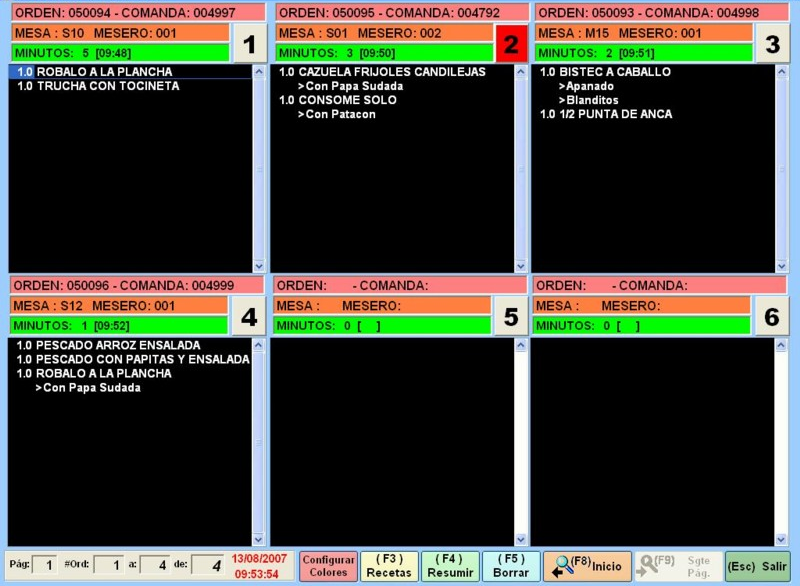
\includegraphics[width=0.8\textwidth]{kitchen.png}
        \caption{Monitor de comandas de la aplicación \emph{RestBar}
        \cite{bib:restBar}.}
        \label{fig:kitchen}
      \end{center}
    \end{figure}
    
    La aplicación muestra qué camarero ha solicitado el plato, la hora en que
    lo solicitó y los minutos que han pasado desde que lo hizo. Cuando los
    productos están listos para servir, los cocineros informan a los
    camareros cambiando el estado del pedido a través de la aplicación.

    \item Si el restaurante tiene entre sus servicios el reparto a
    domicilio, no está demás que la aplicación cuente con una funcionalidad
    en la que quede constancia de los pedidos a domicilio que tiene pendientes
    (figura \ref{fig:deliveries}):

    \begin{figure}[!h]
      \begin{center}
        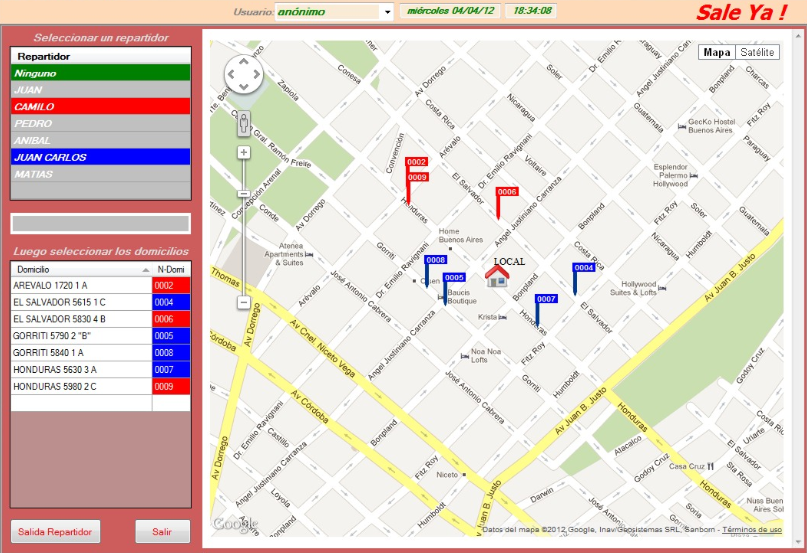
\includegraphics[width=0.8\textwidth]{deliveries.png}
        \caption{Módulo que gestiona los repartos a domicilio. \emph{SaleYa}
        \cite{bib:saleYa}.}
        \label{fig:deliveries}
      \end{center}
    \end{figure}

    La aplicación registra cuáles son los pedidos pendientes, qué repartidor
    se encargará de atenderlos y dónde están los puntos de entrega.
    \end{itemize}

    El abanico de programas de gestión de restaurantes es muy diverso. A la
    hora de adquirir uno u otro conviene determinar bien qué necesidades de
    información se deben satisfacer, de tal forma que no se eche ninguna
    funcionalidad en falta y que no se tengan funcionalidades incompatibles
    con el modelo de negocio que se posee.

    \subsubsection{Gestión de pedidos a través de dispositivos móviles}
    Las soluciones vistas en el apartado anterior van encaminadas a
    facilitar las tareas propias de los camareros y cocineros del restaurante,
    pero en ninguna de ellas se tiene en cuenta al cliente. Si el cliente es
    capaz de realizar pedidos sin necesidad de avisar a un camarero, este
    quedará liberado para realizar otras tareas.

    A continuación, se presentan dos soluciones comerciales que buscan
    satisfacer este objetivo:

    \begin{itemize}
    \item \textbf{vMenu}. Es un sistema ideado por la empresa \emph{Vloo} que
    trata de reinventar la carta tradicional adentrándose en el mundo
    interactivo actual, a través de las pantallas táctiles. Los clientes
    disponen de un dispositivo (\emph{iPad}, tablet o pantalla) en la que
    pueden ver los platos disponibles y realizar los pedidos (figura
    \ref{fig:starters}).

    \begin{figure}[!h]
      \begin{center}
        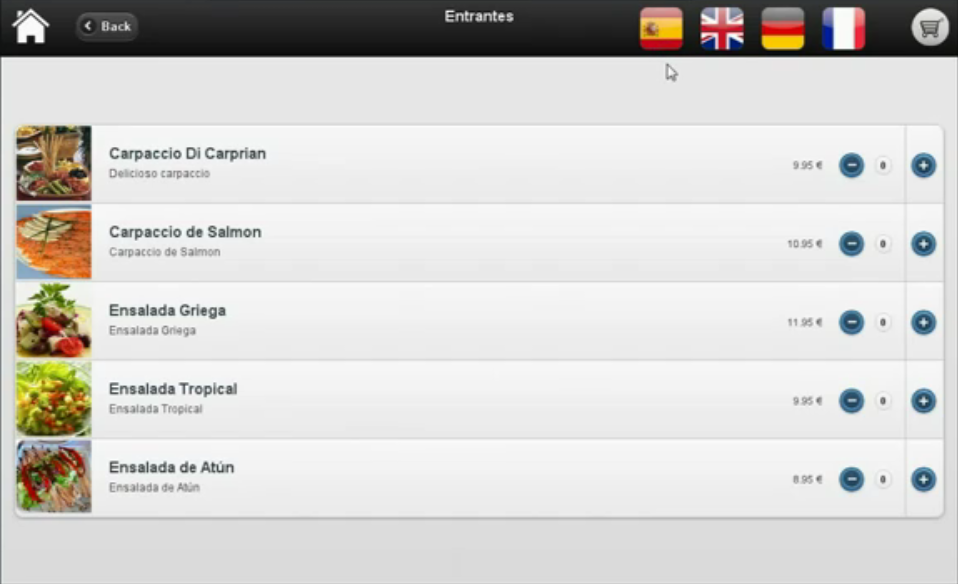
\includegraphics[width=0.8\textwidth]{starters.png}
        \caption{Lista de productos \emph{entrantes}.}
        \label{fig:starters}
      \end{center}
    \end{figure}

    Los productos aparecen distribuidos por categorías y son actualizados
    de manera instantánea. Además, los alimentos son mostrados de una forma
    más atractiva: con fotos, ingredientes, recetas, calorías, preparación y 
    otros datos de interés; y siempre en el idioma del comensal (figura
    \ref{fig:meat}).

    \begin{figure}[!h]
      \begin{center}
        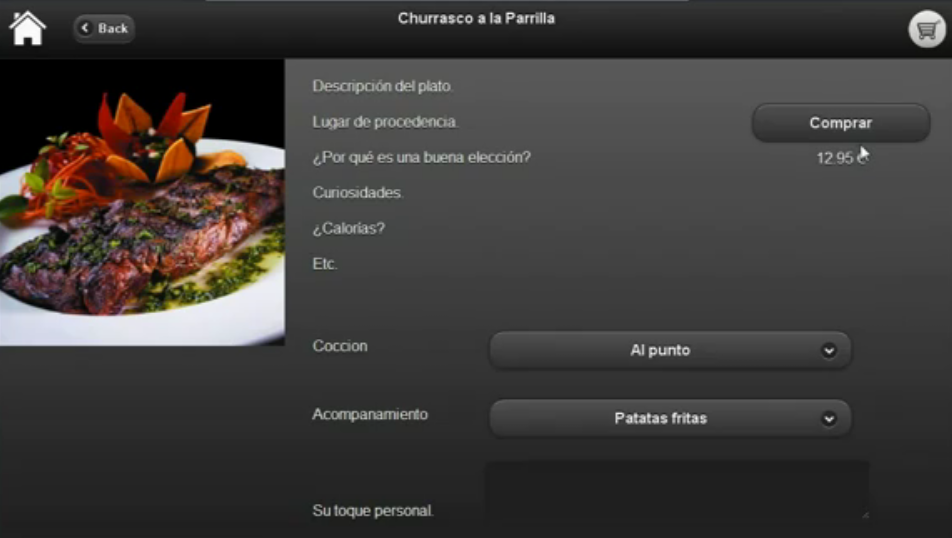
\includegraphics[width=0.8\textwidth]{meat.png}
        \caption{Información asociada al \emph{churrasco a la parrilla}.}
        \label{fig:meat}
      \end{center}
    \end{figure}
    
    \emph{vMenu} reduce los tiempos de espera porque el cliente no necesita
    al camarero para conocer los productos, las recomendaciones o las ofertas
    disponibles; ni para realizar el pedido (figura \ref{fig:order}) o
    solicitar la cuenta; y en caso de necesitarlo, dispone de una opción para
    llamarlo desde el terminal.

    \begin{figure}[!h]
      \begin{center}
        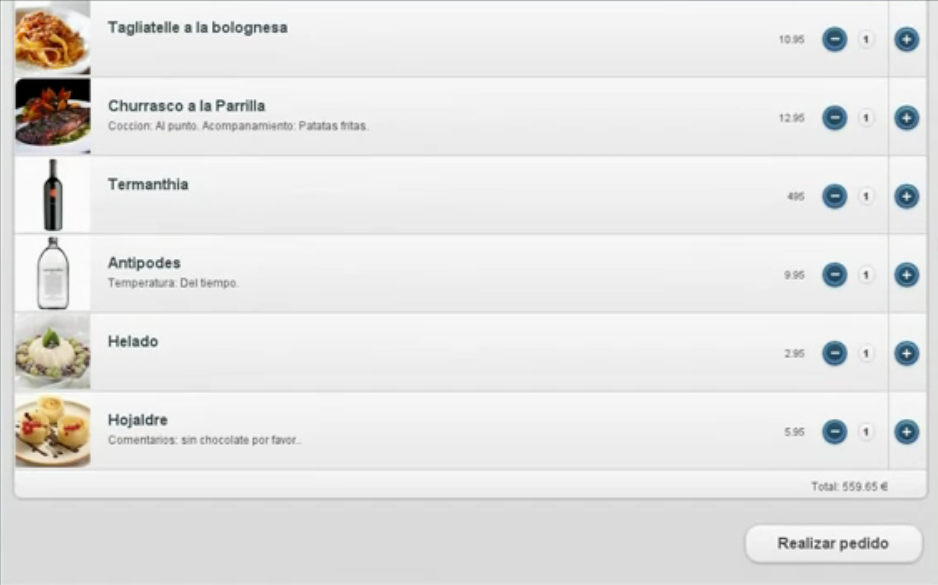
\includegraphics[width=0.8\textwidth]{order.png}
        \caption{Lista de productos elegidos para un pedido.}
        \label{fig:order}
      \end{center}
    \end{figure}

    Por último, a parte de esta función de recogida de pedidos, \emph{vMenu} 
    dispone de todo un sistema integral que permite gestionar las operaciones
    básicas de un restaurante\cite{bib:VMENU}.

    \item \textbf{Brand Table}. \emph{S-Digital}, una \emph{start-up} de la
    Universidad de Sidney, ofrece este prototipo conceptual de mesa de
    restaurante en torno a la cual se distribuyen varios menús electrónicos con
    los que se puede interactuar utilizando un dispositivo móvil con \acs{NFC},
    (figura \ref{fig:brandTable}) de forma que los comensales que se reúnan a 
    su alrededor puedan seleccionar su comida favorita y pagarla
    \emph{in situ} (utilizando \emph{Google Wallet} o \emph{Paypal Mobile}), 
    sin necesidad de tener que esperar a ningún camarero que les tome nota del 
    pedido (figura \ref{fig:brandTableDemo}).

    \begin{figure}[!h]
      \begin{center}
        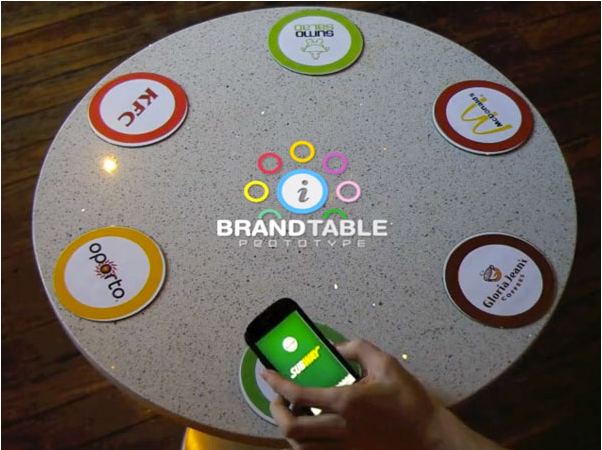
\includegraphics[width=0.8\textwidth]{brandTable.png}
        \caption{Prototipo conceptual de la mesa \emph{Brand Table}.}
        \label{fig:brandTable}
      \end{center}
    \end{figure}

    \begin{figure}[!h]
      \begin{center}
        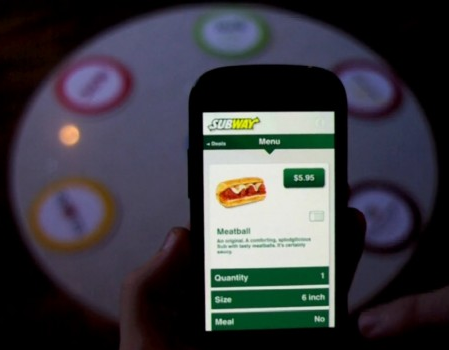
\includegraphics[width=0.8\textwidth]{brandTableDemo.png}
        \caption{Selección de uno de los productos del restaurante
        \emph{Subway}.}
        \label{fig:brandTableDemo}
      \end{center}
    \end{figure}

    Cuando el pedido está preparado, el cliente se levanta y va a recogerlo.
    
    Este sistema está pensado para restaurantes de comida rápida y elimina
    completamente la labor del camarero\cite{bib:brandTable}.
    \end{itemize}


% Local Variables:
%   coding: utf-8
%   mode: latex
%   mode: flyspell
%   ispell-local-dictionary: "castellano8"
% End:
